
\documentclass[11pt]{article}

\usepackage{common}
\usepackage{hyperref}
\title{HW1: Sentiment Classification}
\author{Jonah Philion \\ jonahphilion@college.harvard.edu \\ \href{https://github.com/jonahthelion/cs287-s18/tree/master/HW1}{github}}
\begin{document}

\maketitle{}
\section{Introduction}

In this problem set, we attempt to classify movie reviews as positive or negative. All models investigated take the form of
$$ p(y_i) = \sigma(W\phi(x) + b)$$
where $p(y_i)$ is the probability a review $x$ is negative. The models studied are
\begin{itemize}
\item naive bayes
\item logistic regression with ``bag of words" features
\item multi-layer perceptron with ``continuous bag of words" features
\item convolutional neural net
\end{itemize}
And just for fun
\begin{itemize}
\item Fine-tuning ResNet classifier on images of text
\end{itemize}

%This note lays out our expectation for a homework submission in
%\textit{CS287: Statistical Natural Language Processing}. While you do
%not have to follow this template to the letter, we do expect that
%write-ups have a very clear structure and cover all the elements
%described in this note. With this in mind, the burden is on the
%presenter to demonstrate why deviations from the standard are
%necessary.
%
%All write-ups should include a short introduction. In this section you
%should summarize the underlying problem in high-level language and
%describe the extensions that you have decided to propose in your
%implementation. When you describe these extensions you should
%carefully cite the papers of interest. For instance, it will often be
%useful to cite the work seen in class
%\citep{murphy2012machine}. Alternatively, you can also cite papers
%inline, for instance the work of \citet{berger1996maximum}.


\section{Problem Description}

For all models, a sentence $\boldx_i$ is encoded as a sequence $x_1,...,x_n$ where each $x_j$ is a one-hot vector of length the vocabulary $\mcV$. The classification $y_i$ associated with $\boldx_i$ is 0 if $\boldx_i$ is positive and 1 if $\boldx_i$ is negative. Embeddings $\mcE$ map a one hot vector $x_j$ to a dense vector of size $d$.

%In general, homeworks will be specified using informal
%language. As part of the assignment, we expect you to write-out a
%definition of the problem and your model in formal language. For this
%class, we will use the following notation:
%
%\begin{itemize}
%\item $\boldb, \boldm$;  bold letters for vectors.
%\item $\boldB, \boldM$;  bold capital letters for matrices.
%\item $\mcB, \mcM$;  script-case for sets.
%\item $b_i, x_i$; lower case for scalars or indexing into vectors.
%\end{itemize}
%
%
%For instance in natural language processing, it is common to use
%discrete sets like $\mcV$ for the vocabulary of the language, or $\mcT$ for a
%tag set of the language.  We might also want one-hot vectors
%representing words. These will be of the type
%$\boldv \in \{0,1\}^{|\mcV|}$. In a note, it is crucial to define the
%types of all variables that are introduced. The problem description is the
%right place to do this.
%
%% NLP is also
%% full of sequences. For instance sentences, $w_1, \ldots, w_N$, where
%% here $N$ is a constant length and $w_i \in \mcV$ for all
%% $i \in \{1, \ldots N\}$. If we pretend sentences are all the same
%% length, we can have scoring function over sentences,
%% $s : \mcV^N \mapsto \reals$.  One might be defined as:
%
%% \[ s(w_1, \ldots, w_N) = \sum_{i = 1}^N p(w_i | w_{i-2}, w_{i-1}), \]
%
%% \noindent where $p$ is the bigram probability, which we will cover later in the class.

\section{Model and Algorithms}

All models are trained on the \href{https://nlp.stanford.edu/~socherr/EMNLP2013_RNTN.pdf}{Stanford Sentiment Treebank} (SST1). Unless otherwise specified, models requiring gradient descent are trained with an Adam optimizer of learning rate 0.001 and weight decay 0.0005.  Training loss and validation loss are recorded in real time with \href{https://github.com/facebookresearch/visdom}{visdom}.

%Here you specify the model itself. This section should formally
%describe the model used to solve the task proposed in the previous
%section. This section should try to avoid introducing new vocabulary
%or notation, when possible use the notation from the previous section.
%Feel free to use the notation from class, but try to make the note
%understandable as a standalone piece of text.
%
%This section is also a great place to include other material that
%describes the underlying structure and choices of your model, for
%instance here are some example tables and algorithms from full
%research papers:
%
%
%
%\begin{itemize}
%\item diagrams of your model,
%
%  \begin{center}
%    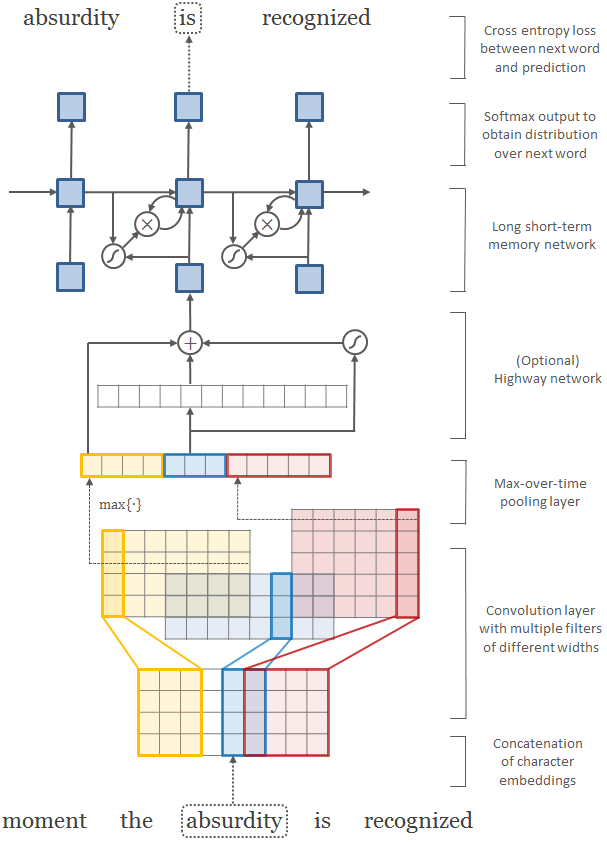
\includegraphics[width=0.4\textwidth]{network}
%  \end{center}
%\item feature tables,
%
%  \begin{center}
%    \begin{tabular}{@{}lll@{}}
%      \toprule
%      &\multicolumn{2}{c}{Mention Features  } \\
%      & Feature & Value Set\\
%      \midrule
%      & Mention Head & $\mcV$ \\
%      & Mention First Word & $\mcV$ \\
%      & Mention Last Word & $\mcV$ \\
%      & Word Preceding Mention & $\mcV$ \\
%      & Word Following Mention & $\mcV$\\
%      & \# Words in Mention & $\{1, 2, \ldots \}$ \\
%      & Mention Type & $\mathcal{T}$ \\
%      \bottomrule
%    \end{tabular}
%  \end{center}
%
%\item pseudo-code,
%
%  \begin{algorithmic}[1]
%    \Procedure{Linearize}{$x_1\ldots x_N$, $K$, $g$}
%    \State{$B_0 \gets \langle (\langle \rangle, \{1, \ldots, N\}, 0, \boldh_0, \mathbf{0})  \rangle$}
%    \For{$m = 0, \ldots, M-1$ }
%    \For{$k = 1, \ldots, |B_m|$}
%    \For{$i \in \mcR$}
%    \State{$(y, \mcR, s, \boldh) \gets \mathrm{copy}(B_m^{(k)})$}
%    \For{word $w$ in phrase $x_i$}
%    \State{$y \gets y $ append $w$ }
%    \State{$s \gets s + \log q(w, \boldh) $ }
%    \State{$\boldh \gets \delta(w, \boldh)$}
%    \EndFor{}
%    \State{$B_{m+|w_i|} \gets B_{m+|w_i|} + (y, \mcR - i, s,   \boldh)$}
%    \State{keep top-$K$ of $B_{m+|w_i|}$ by $f(x, y) + g(\mcR)$}
%    \EndFor{}
%    \EndFor{}
%    \EndFor{}
%    \State{\Return{$B_{M}^{(k)}$}}
%    \EndProcedure{}
%  \end{algorithmic}
%
%\end{itemize}


\section{Experiments}

\begin{subsection}{Naive Bayes}
All words for both labels are initialized to a count of $\alpha$. Figure \ref{fig:clusters} shows that performance of the algorithm on the validation set is robust to changes in $\alpha$. With $\alpha=.5$, performance on the test set using binarized and count word vectors are analyzed in Table \ref{tab:nb}.\\
The weight vector determined by Naive Bayes can be interpreted as the sentiment associated with particular words. The most positive and most negative words and their weights for binarized bag of words are shown in Table \ref{tab:bnwords}.



\begin{figure}
  \centering
  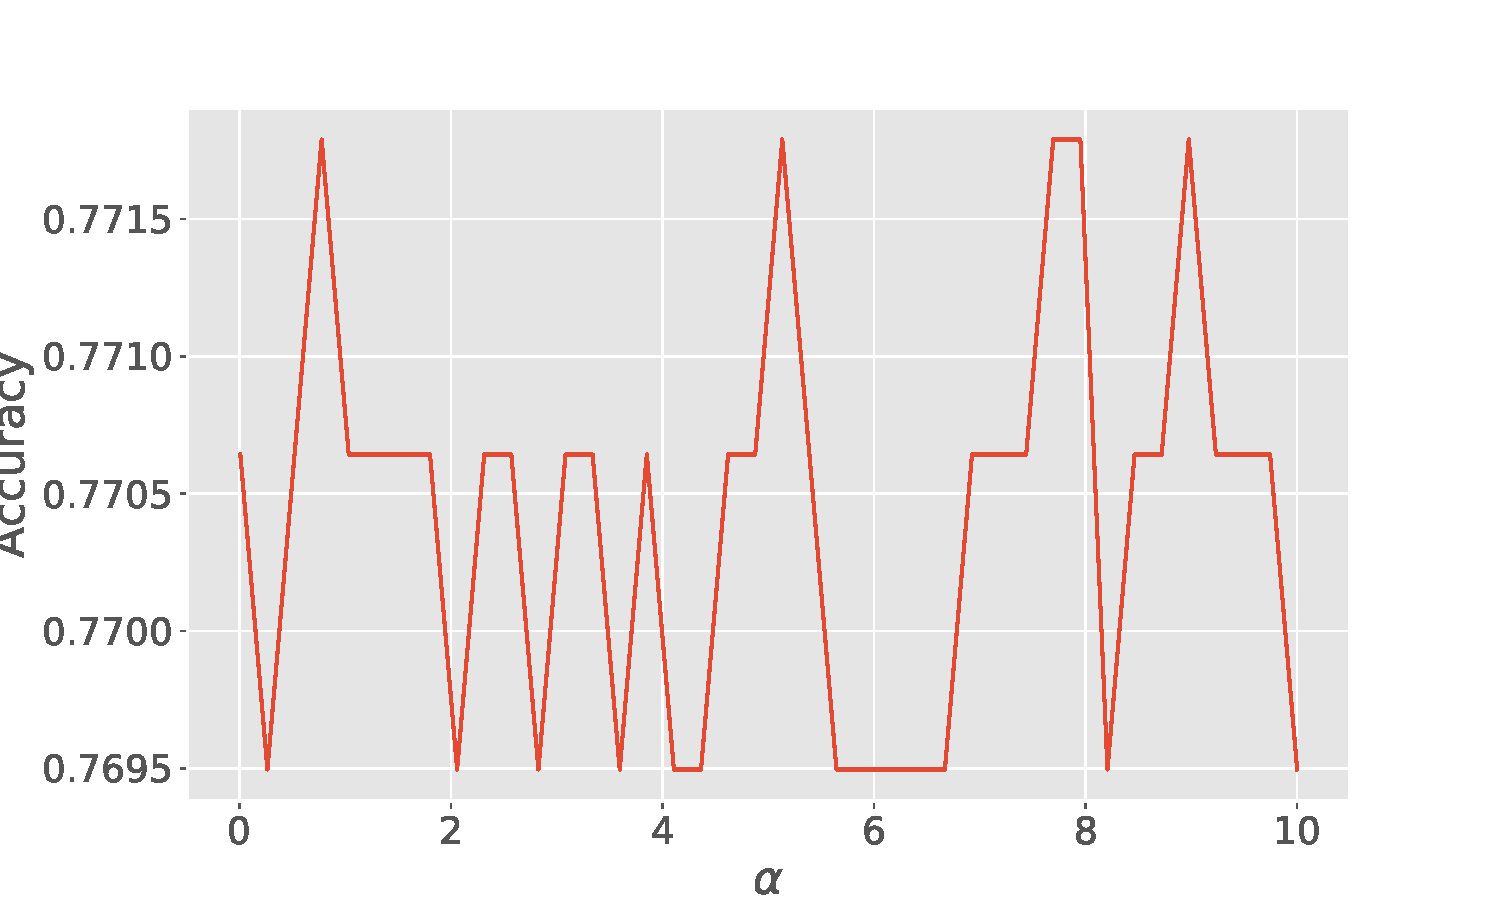
\includegraphics[width=6cm]{imgs/alpha}
  \caption{\label{fig:clusters} Affect of global smoothing parameter $\alpha$ on validation accuracy. Validation accuracy is calculated using sklearn's \texttt{accuracy\_score}. The performance is not sensitive to $\alpha$.}
\end{figure}

\begin{table}[h]
\centering
\begin{tabular}{llrrr}
 \toprule
 Model &  & Acc. & Bce. & Roc.\\
 \midrule
 \textsc{Binarized} & & 0.791 & 0.679 & 0.867\\
 \textsc{Counts} & & 0.793  & 0.686 & 0.867\\
 \bottomrule
\end{tabular}
\caption{\label{tab:nb} Binarizing or counting words does not significantly affect the performance of the model on the test set.}
\end{table}



\begin{table}[h]
\centering
\begin{tabular}{cccccccccc}
 \midrule
 stupid & unfunny& pointless  & poorly & suffers & Feels & tiresome & car \\
   5.39452 & 5.1085& 5.03998 &4.96641&4.96641 & 4.88701 & 4.88701 & 4.88701 \\
 \bottomrule
 \bottomrule
 powerful  & solid& perfectly & inventive & refreshing & riveting & wonderfully & universal \\
  -5.79766 & -5.7109 & -4.99019 & -4.85754 & -4.78398 & -4.70458 & -4.61832 & -4.61832 \\
 \bottomrule
\end{tabular}
\caption{\label{tab:nbwords} Words with the highest and lowest weights in the naive bayes weight vector agree with intuition for being negative and positive words respectively.}
\end{table}

\end{subsection}




\begin{subsection}{Logistic Regression}
In the logistic regression model, we take the bag of words $\phi(x)$ but train $w$ and $b$ instead of calculating $w$ and $b$. Figure \ref{fig:logtrain} shows that as the model decreases cross entropy, the accuracy on the validation set also increases. However, this model does not do significantly better than naive bayes. The model is trained with batch size of 150 for 150 iterations with an adam optimizer of learning rate 0.0002 and weight decay 0.0005. The weight vector is initialized to zero to guard against words in the validation set which are not in the training set. The model is trained on binary and count vectors as with naive bayes. The metrics are recorded in Table \ref{tab:logreg}. Significant words are recorded in Table \ref{tab:logwords}.


\begin{figure}
  \centering
  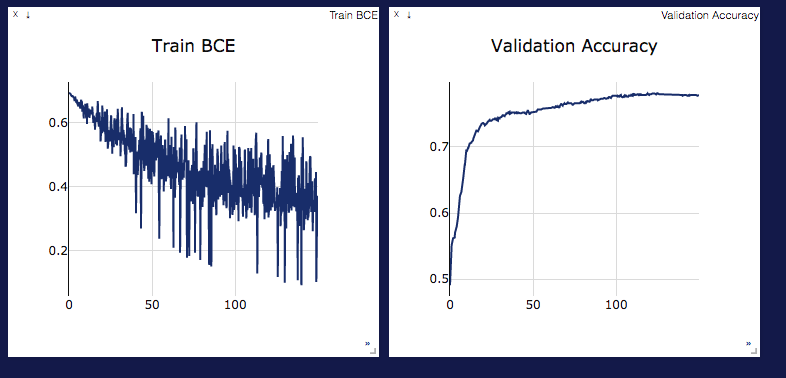
\includegraphics[width=6cm]{imgs/logtrain}
  \caption{\label{fig:logtrain} The left is the binary cross entropy recorded during training of binarized logistic regression and the right is the classification accuracy tracked during training. The objective function is tightly correlated with classification accuracy. The model is no better than naive bayes.}
\end{figure}

\begin{table}[h]
\centering
\begin{tabular}{llrrr}
 \toprule
 Model &  & Acc. & Bce. & Roc.\\
 \midrule
 \textsc{Binarized} & & 0.789 & 0.496 & 0.876\\
 \textsc{Counts} & & 0.789  & 0.497 & 0.873\\
 \bottomrule
\end{tabular}
\caption{\label{tab:logreg} Binarizing or counting words does not significantly affect the performance of the model on the test set.}
\end{table}


\begin{table}[h]
\centering
\begin{tabular}{cccccccccc}
 \midrule
bad & dull & mess  & worst & too &flat & stupid&? \\
   0.772932 & 0.687341& 0.657265 &0.648685&0.645756&0.611209 & 0.575218 &  0.572873 \\
 \bottomrule
 \bottomrule
 solid  & fun& best & powerful & entertaining & heart & fascinating & love \\
  -0.689454 & -0.672897& -0.6613 & -0.657444 & -0.591135 &  -0.586589 &-0.578906 & -0.574162 \\
 \bottomrule
\end{tabular}
\caption{\label{tab:logwords} Words with the highest and lowest weights in the logistic regression weight vector agree with intuition for being negative and positive words respectively. There is some overlap with naive bayes.}
\end{table}

\end{subsection}




\begin{subsection}{Continuous bag of Words}

In the Continuous bag of words (CBOW) model, one-hot vectors $x_i$ for each word are mapped to a dense vector by ab embedding $\mcE$ in a lower dimensional feature space. These lower dimensional vectors are then summed or averaged. The order of the words is therefore lost during the transformation $\phi(\boldx_i)$ as it is in the naive bayes model. The model is trained with an Adam optimizer of learning rate 0.00002 and batch size 100 for 350 epochs. The embedding is initialized to AWS word vectors but allowed to change during training. The embeddings improve the accuracy of the model over logistic regression and naive bayes as shown in Table $\ref{tab:cbowtab}$ regardless of whether sum or max pooling is used. Figure \ref{fig:cbowfit} shows the objective and validation accuracy during training of the model with max pooling.

\begin{table}[h]
\centering
\begin{tabular}{llrrr}
 \toprule
 Model &  & Acc. & Bce. & Roc.\\
 \midrule
 \textsc{Mean} & & 0.824 & 0.416 & 0.898\\
 \textsc{Sum} & & 0.816  & 0.448 & 0.886\\
  \textsc{Max} & & 0.798  & 0.447 & 0.880\\
 \bottomrule
\end{tabular}
\caption{\label{tab:cbowtab} The word vectors improve the accuracy of the model.}
\end{table}

\begin{figure}
  \centering
  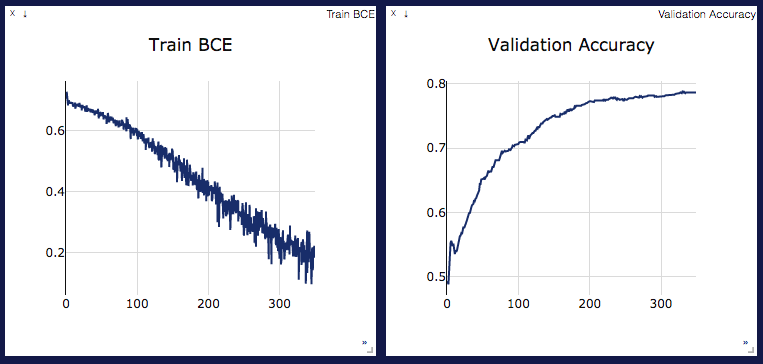
\includegraphics[width=6cm]{imgs/cbowtrain}
  \caption{\label{fig:logtrain} The left is the binary cross entropy recorded during training of CBOW and the right is the classification accuracy tracked during training. The objective function is tightly correlated with classification accuracy. The model is significantly better than naive bayes.}
\end{figure}

\end{subsection}


\begin{subsection}{CNN}

Following \href{http://aclweb.org/anthology/D/D14/D14-1181.pdf}{Yoon's CNN paper}, we train a simple CNN with one layer of convolution. The convolution layer includes

\begin{itemize}
\item 300$\rightarrow$ 50, kernel 3, stride 1, padding 1
\item 300$\rightarrow$ 25, kernel 4, stride 1, padding 1
\item 300$\rightarrow$ 25, kernel 5, stride 1, padding 1
\end{itemize}

Each convolution layer consists of the convolution, then ReLU, then single output max pool. We concatenate the resultant features and output a fully connected layer with 0.5 dropout. As an experiment, we train first using the wikipedia 300d embedding and second using the GloVe 6B 300d embedding. The optimizer is an Adam optimizer of learning rate .00006 in both cases. We treat the embeddings as fixed. The model is trained for 150 epochs with batch size 50. Training and validation metrics tracked during training are shown in Figure \ref{fig:conv}.

\begin{figure}
  \centering
  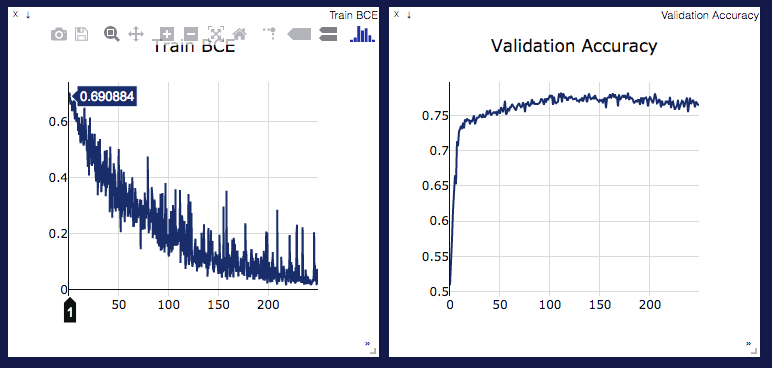
\includegraphics[width=6cm]{imgs/convtrain}
  \caption{\label{fig:logtrain} The left is the binary cross entropy recorded during training of Conv net with wikipedia word embeddings and the right is the classification accuracy tracked during training. The objective function is tightly correlated with classification accuracy. The model is significantly better than naive bayes.}
\end{figure}

\end{subsection}





\begin{subsection}{ResNet}

\end{subsection}






%Finally we end with the experimental section. Each assignment will make clear the main experiments and baselines that you should run. For these experiments you should present a main results table. Here we give a sample Table~\ref{tab:results}. In addition to these results you should describe in words what the table shows and the relative performance of the models.
%
%Besides the main results we will also ask you to present other results
%comparing particular aspects of the models. For instance, for word
%embedding experiments, we may ask you to show a chart of the projected
%word vectors. This experiment will lead to something like
%Figure~\ref{fig:clusters}. This should also be described within the
%body of the text itself.
%
%
%\begin{table}[h]
%\centering
%\begin{tabular}{llr}
% \toprule
% Model &  & Acc. \\
% \midrule
% \textsc{Baseline 1} & & 0.45\\
% \textsc{Baseline 2} & & 2.59 \\
% \textsc{Model 1} & & 10.59  \\
% \textsc{Model 2} & &13.42 \\
% \textsc{Model 3} & & 7.49\\
% \bottomrule
%\end{tabular}
%\caption{\label{tab:results} Table with the main results.}
%\end{table}
%
%
%\begin{figure}
%  \centering
%  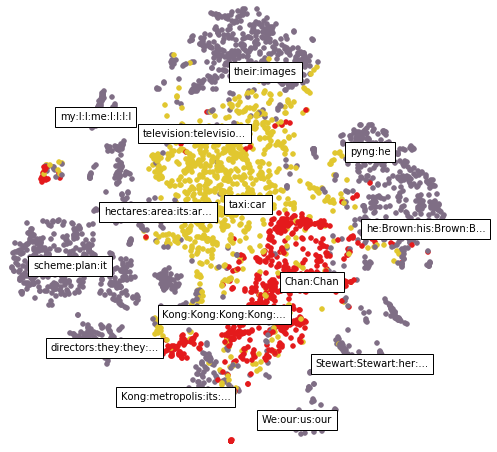
\includegraphics[width=6cm]{cluster_viz}
%  \caption{\label{fig:clusters} Sample qualitative chart.}
%\end{figure}


\section{Conclusion}

End the write-up with a very short recap of the main experiments and the main results. Describe any challenges you may have faced, and what could have been improved in the model.

\bibliographystyle{apalike}
\bibliography{writeup}

\end{document}
